% This LaTeX was auto-generated from MATLAB code.
% To make changes, update the MATLAB code and export to LaTeX again.

\sloppy
\epstopdfsetup{outdir=./}
\graphicspath{ {./5ef/assignment1task5ef_images/} }

\begin{matlabcode}
% initialize the values
x_bar = zeros(2,1)
\end{matlabcode}
\begin{matlaboutput}
x_bar =
     0
     0

\end{matlaboutput}
\begin{matlabcode}
P = 25 * eye(2)
\end{matlabcode}
\begin{matlaboutput}
P =
    25     0
     0    25

\end{matlaboutput}
\begin{matlabcode}

H_r = eye(2)
\end{matlabcode}
\begin{matlaboutput}
H_r =
     1     0
     0     1

\end{matlaboutput}
\begin{matlabcode}
H_c = eye(2)
\end{matlabcode}
\begin{matlaboutput}
H_c =
     1     0
     0     1

\end{matlaboutput}
\begin{matlabcode}

R_c = [79, 36; 36, 36]
\end{matlabcode}
\begin{matlaboutput}
R_c =
    79    36
    36    36

\end{matlaboutput}
\begin{matlabcode}
R_r = [28, 4; 4, 22]
\end{matlabcode}
\begin{matlaboutput}
R_r =
    28     4
     4    22

\end{matlaboutput}
\begin{matlabcode}

z_c = [2; 14]
\end{matlabcode}
\begin{matlaboutput}
z_c =
     2
    14

\end{matlaboutput}
\begin{matlabcode}
z_r = [-4; 6]
\end{matlabcode}
\begin{matlaboutput}
z_r =
    -4
     6

\end{matlaboutput}
\begin{matlabcode}

% set up for plotting ellipses
Npts = 100; % number of points around the circle
circle = [cos( 0:(2*pi/Npts):(2*pi) ); sin( 0:(2*pi/Npts):(2*pi) )];

% initial 1 sigma ellipses
figure(1); clf; hold on; grid on;
data = x_bar + chol(P)' * circle;
plot(data(1,:), data(2, :), 'DisplayName','prior')

% measurements
scatter(z_c(1), z_c(2), 'DisplayName', 'z_c')
scatter(z_r(1), z_r(2), 'DisplayName', 'z_r')

legend()
\end{matlabcode}
\begin{center}
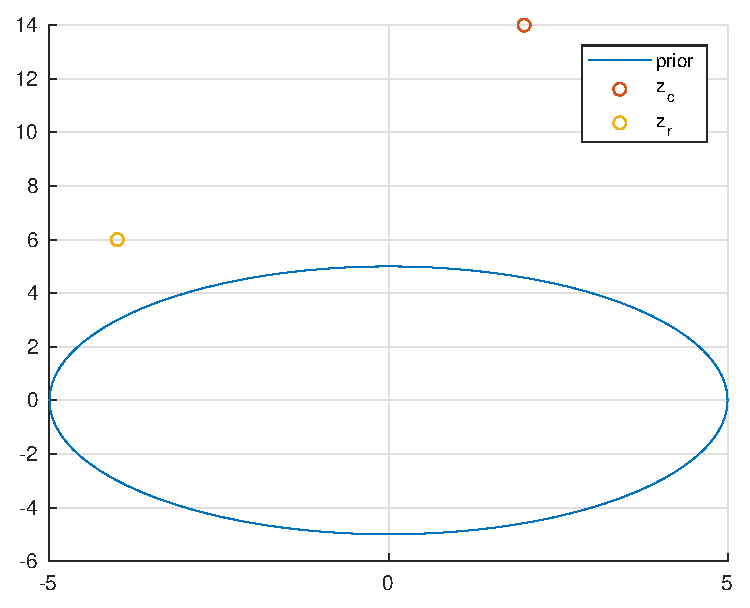
\includegraphics[width=\maxwidth{56.196688409433015em}]{figure_0}
\end{center}


\begin{matlabcode}
% You can make some functions to ease the conditionioning
% FILL IN THE DOTS ...
condition_mean = @(x_bar, z, P, H, R) x_bar + P*(H*P*H' + R)^(-1)*(z-x_bar);
condition_cov = @(P, H, R) P - H*P*(H*P*H' + R)^(-1)*P*H';
\end{matlabcode}


\begin{matlabcode}
% task 5 (f)
% FILL IN FOR THE DOTS ...

% condition on camera
x_bar_c = condition_mean(x_bar, z_c, P, H_c, R_c)
\end{matlabcode}
\begin{matlaboutput}
x_bar_c =
   -1.8918
    6.8542

\end{matlaboutput}
\begin{matlabcode}
P_c = condition_cov(P, H_c, R_c)
\end{matlabcode}
\begin{matlaboutput}
P_c =
   17.4475    4.4572
    4.4572   12.1236

\end{matlaboutput}
\begin{matlabcode}

% condition on radar
x_bar_r = condition_mean(x_bar, z_r, P, H_r, R_r)
\end{matlabcode}
\begin{matlaboutput}
x_bar_r =
   -2.1414
    3.3737

\end{matlaboutput}
\begin{matlabcode}
P_r = condition_cov(P, H_r, R_r)
\end{matlabcode}
\begin{matlaboutput}
P_r =
   13.1313    1.0101
    1.0101   11.6162

\end{matlaboutput}
\begin{matlabcode}

% Plot 1 sigma ellipses
figure(2); clf; hold on; grid on;

data = x_bar + chol(P)' * circle;
plot(data(1,:), data(2, :), 'DisplayName','prior')

data = x_bar_c + chol(P_c)' * circle;
plot(data(1,:), data(2, :), 'DisplayName', 'c')

data = x_bar_r + chol(P_r)' * circle;
plot(data(1,:), data(2, :), 'DisplayName', 'r')

% measurements
scatter(z_c(1), z_c(2), 'DisplayName', 'z_c')
scatter(z_r(1), z_r(2), 'DisplayName', 'z_r')
legend()
\end{matlabcode}
\begin{center}
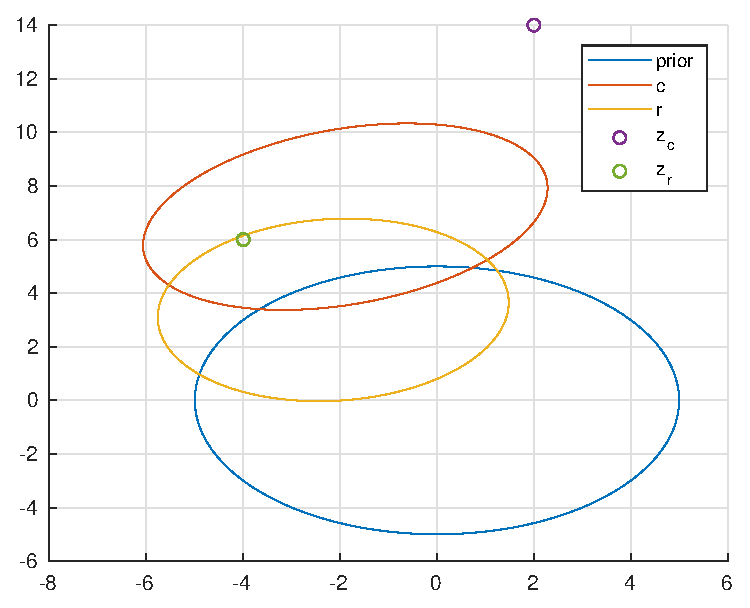
\includegraphics[width=\maxwidth{56.196688409433015em}]{figure_1}
\end{center}


\begin{matlabcode}
% task 5 (g)

% condition the already camera conditioned on the radar
x_bar_cr = condition_mean(x_bar_c, z_r, P_c, H_r, R_r)
\end{matlabcode}
\begin{matlaboutput}
x_bar_cr =
   -2.7183
    6.4872

\end{matlaboutput}
\begin{matlabcode}
P_cr =  condition_cov(P_c, H_r, R_r)
\end{matlabcode}
\begin{matlaboutput}
P_cr =
   10.7043    2.3261
    2.3261    7.7676

\end{matlaboutput}
\begin{matlabcode}

% condition the already radar conditioned on the camera
x_bar_rc = condition_mean(x_bar_r, z_c, P_r, H_c, R_c)
\end{matlabcode}
\begin{matlaboutput}
x_bar_rc =
   -2.7183
    6.4872

\end{matlaboutput}
\begin{matlabcode}
P_rc = condition_cov(P_r, H_c, R_c)
\end{matlabcode}
\begin{matlaboutput}
P_rc =
   10.7043    2.3261
    2.3261    7.7676

\end{matlaboutput}
\begin{matlabcode}

% Plot 1 sigma ellipses
figure(3); clf; hold on; grid on;

data = x_bar + chol(P)' * circle;
plot(data(1,:), data(2, :), 'DisplayName','prior')

data = x_bar_c + chol(P_c)' * circle;
plot(data(1,:), data(2, :), 'DisplayName', 'c')

data = x_bar_r + chol(P_r)' * circle;
plot(data(1,:), data(2, :), 'DisplayName', 'r')

data = x_bar_cr + chol(P_c)' * circle;
plot(data(1,:), data(2, :), 'DisplayName', 'cr')

data = x_bar_rc + chol(P_r)' * circle;
plot(data(1,:), data(2, :), 'DisplayName', 'rc')

% meausrements
scatter(z_c(1), z_c(2), 'DisplayName', 'z_c')
scatter(z_r(1), z_r(2), 'DisplayName', 'z_r')

legend()
\end{matlabcode}
\begin{center}
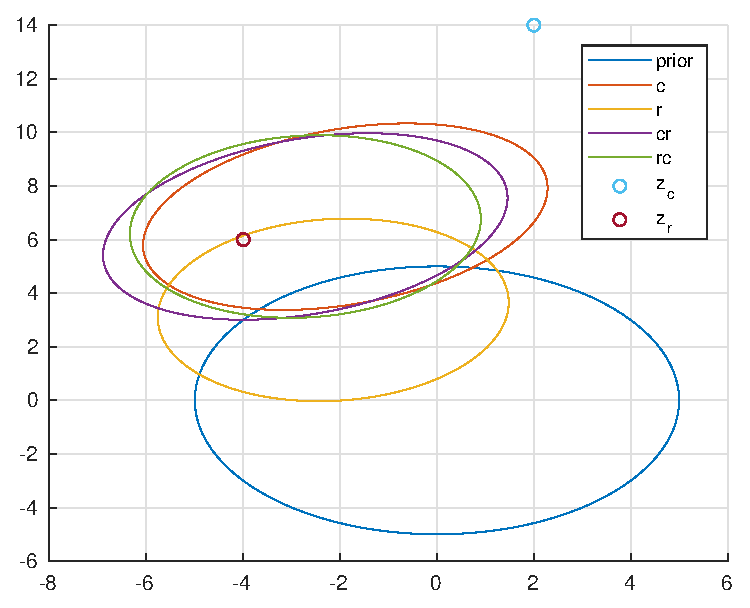
\includegraphics[width=\maxwidth{56.196688409433015em}]{figure_2}
\end{center}
